\section{Document Stores}
\subsection{Einleitung}
Document-Stores speichern strukturierte Daten in Datensätzen, die Dokumente genannt werden. Grundsätzlich vereinigen sie die Schemafreiheit von Key-Value-Stores mit der Möglichkeit zur Strukturierung der gespeicherten Daten. Somit lassen sich Document-Stores als Erweiterung von Key-Value Stores betrachten. Vorteil hierbei ist, dass es bei Document-Stores im Gegensatz zu Key-Value Stores möglich ist komplexere auf den Inhalt (die Attribute) der Dokumente gerichtete Abfragen zu stellen. Dies ist bei Key-Value-Stores nicht möglich.

\subsection{Eigenschaften}
Die Kerneigenschaften der Document-Stores sind:
\begin{itemize}
\item Daten in Form von Dokumenten
\item Dokumente sind Schemalos
\item Horizontale Verteilung
\end{itemize}
Bei der Betrachtung von Document-Stores bezieht sich das Wort "document" auf die hierarchische Struktur der abgespeicherten Daten. Die hier betrachteten Dokumente bestehen jedoch lediglich aus binären Daten oder einfachem Text. Ferner kann es sich um Semi-strukturierte Daten wie JSON oder XML handeln. Während ältere Document-Stores auf XML setzten, ist bei neueren Document-Stores das JSON ähnliche BSON üblich. 


\subsection{Datenmodell}
Im Zentrum des Datenmodells der Document-Stores stehen die Documents, die eine hierarchische Struktur aufweisen. So kann ein Dokument auf viele weitere Dokumente verweisen. Dies ist möglich, da ein Dokument Listen enthalten kann. 
\\
Die Dokumente liegen üblicherweise in JSON bzw. BSON vor.

\subsubsection{JSON}
Die Java-Script-Object-Notation ist ein vom Menschen und Maschinen lesbarer Standard zur Beschreibung von Daten. JSON ist wie XML ein Standard zum Datenaustausch im Web.
\begin{figure}
	\centering
	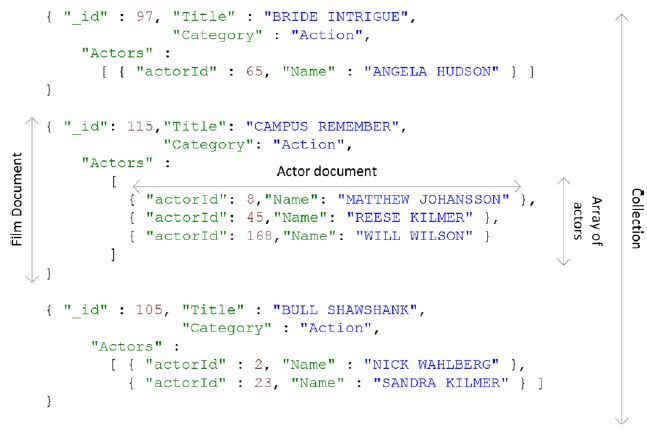
\includegraphics[scale=0.5]{images/docstores_1.jpg}
	\caption{Beispiel eines JSON-Dokuments}\label{fig:doc1}
\end{figure}
In \ref{fig:doc1} ist ein Beispiel für ein JSON-Dokument zu sehen. Vorteil von JSON ist, dass JSON-Dokumente einfach zu zerlegen und umzuwandeln sind. Dies verringert den Aufwand, der in der Anwendungsschicht betrieben werden muss.
\subsubsection{BSON}
Unter BSON sind binär kodierte JSON-Dokumente zu verstehen. BSON erweitert das Modell von JSON um weitere Datentypen und ermöglicht effizientes kodieren und dekodieren innerhalb verschiedener Sprachen.
\subsection{Anwendungsfälle}
JSON basierte Document-Stores haben vor allem in Web-basierten Anwendungen ihre Vorzüge. Hier wird häufig JSON als Datenschicht verwendet, weswegen Document-Stores hier bevorzugt werden.
\\
XML-basierte Document-Stores finden vor allem in Content-Management-Systemen Anwendung, da sie hier ein Management Repository für XML-basierte Textdateien zur Verfügung stellen.
\subsection{Bewertung}
